\addcontentsline{toc}{chapter}{Занятие 3. Классическое определение вероятности}
\chapter*{Занятие 3. Классическое определение вероятности}

\addcontentsline{toc}{section}{Контрольные вопросы и задания}
\section*{Контрольные вопросы и задания}

\subsubsection*{Приведите определение вероятностного эксперимента, вероятностного пространства, случайного события.}

Вероятностным экспериментом называется явление, исход которого для нас не определён, и который можно повторить любое число раз независимым образом.

Вероятностное пространство --- совокупность всех исходов вероятностного эксперимента, $\Omega$.

Случайное событие --- подмножество всех исходов вероятностного эксперимента.

\subsubsection*{Как вычислить вероятность события в случае, когда вероятностное пространство состоит из конечного количества равновероятных элементарных событий?}

В этом случае вероятность любого события A вычисляется по формуле
$$ P(A) =
\frac{ |A| }{ |\Omega| },$$
называемой классическим определением вероятности.

\subsubsection*{Запишите формулу включений и исключений.}

Если
$ B_1, B_2,  \dotsc , B_m $ --- некоторые события, то имеет место равенство
$ P\{ \bigcup \limits_{i=1}^m B_i \} =
\sum \limits_{i=1}^m P \{ B_i \} -
\sum \limits_{ 1 \leq i_1 < i_2 \leq m } \{ B_{ i_1 } \cap B_{ i_2 } \} + \dotsc + \\
+ (-1)^{k-1} \sum \limits_{ 1 \leq i_1 < i_2 < \dotsc < i_k \leq m } P \{ B_{ i_1 } \cap B_{ i_2 } \cap \dotsc \cap B_{ i_k } \} + \dotsc + \\
+ (-1)^{m-1} P \{ B_1 \cap B_2 \cap \dotsc \cap B_m \}.$

\addcontentsline{toc}{section}{Аудиторные задачи}
\section*{Аудиторные задачи}

\subsubsection*{3.3}

\textit{Задание.} Пусть A и B такие события, что
$$P \left( A \cap B \right) = \frac{1}{4},
P \left( \overline{A} \right) = \frac{1}{3},
P \left( B \right) = \frac{1}{2}. $$
Вычислите $P \left( A \cup B \right)$.

\textit{Решение.} Вычислим вероятность события A:
$$P \left( A \right) =
1 - P \left( \overline{A} \right) =
1 - \frac{1}{3} =
\frac{2}{3}.$$

Так как события независимы, то вероятность пересечения событий равна произведению пересечений, т.е
$P \left( A \cap B \right) = P \left( A \right) P \left( B \right) $.

Вычислим вероятность объединения:
$$P \left( A \cup B \right) =
P \left( A \right) + P \left( B \right) - P \left( A \cap B \right) =
\frac{2}{3} + \frac{1}{2} - \frac{1}{4} =
\frac{8+6-3}{12} =
\frac{11}{12}.$$

\subsubsection*{3.4}

\textit{Задание.} Было подброшено три монеты.
Найдите вероятности событий:
\begin{enumerate}[label=\alph*)]
\item A = {хотя бы одна из монет выпала гербом};
\item B = {выпало ровно два герба};
\item C = {выпало не меньше двух гербов}.
\end{enumerate}

\textit{Решение.} На первой монете может появиться или герб, или цифра.
Аналогичные два элементарных исхода возможны при подбрасывании остальных монет.
Таким образом, общее число возможных элементарных исходов испытания равно $2 \cdot 2 \cdot 2 = 8$.
Эти исходы равновероятны.

\begin{enumerate}[label=\alph*)]
\item Благоприятствующие интересующему нас событию
(хотя бы одна из монет выпала гербом)
являются следующие три исхода (<<Г>> означает герб, <<Ц>> --- цифра): 1) ГЦЦ, 2) ГГЦ, 3) ГГГ.

Искомая вероятность равна отношению числа исходов, благоприятствующих событию, к числу всех возможных элементарных исходов:
$$P \left( A \right) =
\frac{3}{8};$$

\item благоприятствующим интересующему нас событию (выпало ровно два герба) является следующий исход: ГГЦ.

Искомая вероятность равна
$$P \left( B \right) =
\frac{1}{8};$$

\item благоприятствующие интересующему нас событию (выпало не меньше двух гербов) являются следующие два исхода: 1) ГГЦ, 2) ГГГ.

Искомая вероятность равна
$$P \left( C \right) =
\frac{2}{8} =
\frac{1}{4}.$$
\end{enumerate}

\subsubsection*{3.5}

\textit{Задание.} Подброшено 12 игральных кубиков.
Найдите вероятность того, что каждое из очков $1, 2, \dotsc, 6$ выпало дважды.

\textit{Решение.}
На выпавшей грани <<первого>> игрального кубика может появиться одно очко, два очка, $ \dotsc $, шесть очков.
Аналогичные шесть элементарных исходов возможны при бросании остальных кубиков.
Таким образом, общее число возможных элементарных исходов испытания равно $6 \cdot 6 \cdot \dotsc \cdot 6 = 6^{12}$.
Эти исходы в силу симметрии кубиков равновероятны.

Благоприятствующим интересующему нас событию
(каждое из очков выпадет дважды)
является $C_{12}^2 \cdot C_{10}^2 \cdot C_8^2 \cdot C_6^2 \cdot C_4^2 \cdot C_2^2$ исходов.

Искомая вероятность равна отношению числа исходов, благоприятствующих событию,
к числу всех возможных элементарных исходов:
$$P =
\frac{C_{12}^2 \cdot C_{10}^2 \cdot C_8^2 \cdot C_6^2 \cdot C_4^2 \cdot C_2^2}{6^{12}}.$$

\subsubsection*{3.6}

\textit{Задание.}
Игральный кубик изготовлено так,
что вероятность выпадения каждой грани пропорциональна количеству очков, изображённой на этой грани.
Вычислите вероятность того, что при подбрасывании такого игрального кубика выпадет чётное количество очков.

\textit{Решение.} Вероятность выпадения единицы пропорциональна единице, т.е. равна n, где n --- любое натуральное число.
Вероятность выпадения двойки равна $2 n$, тройки --- $3 n$, четвёрки --- $4 n$, пятёрки --- $5 n$ и шестёрки --- $6 n$.
Вероятность выпадения хоть какого-то числа равна единице, т.е. сумма вероятностей выпадения всех граней равна единице: $n + 2 n + 3 n + 4 n + 5 n + \\ + 6 n = 21 n = 1$.
Отсюда
$$n =
\frac{1}{21}.$$

Интересующие нас события: выпадет 2 очка, 4 очка или 6 очков.
2 очка может выпасть с вероятностью
$$ P \left( 2 \right) =
2 \cdot \frac{1}{21} =
\frac{2}{21}.$$
4 очка может выпасть с вероятностью
$$ P \left( 4 \right) =
4 \cdot \frac{1}{21} =
\frac{4}{21}.$$
6 очков может выпасть с вероятностью
$$ P \left( 6 \right) =
6 \cdot \frac{1}{21} =
\frac{6}{21}.$$

Вероятность выпадения чётного числа равна сумме вероятностей их выпадения:
$$P \left( 2, 4, 6 \right) =
\frac{2}{21} + \frac{4}{21} + \frac{6}{21} =
\frac{12}{21}.$$

\subsubsection*{3.7}

\textit{Задание.} Найдите вероятность того, что наугад выбранное число из множества $\{ 1, 2, \dotsc, 100!\}$ делится:
\begin{enumerate}[label=\alph*)]
\item на 2;
\item на 2 и на 3;
\item хотя бы на одно из чисел 2, 3, или 5.
\end{enumerate}

\textit{Решение.} Всего чисел $100!$.
\begin{enumerate}[label=\alph*)]
\item На 2 делится каждое второе число, т.е. количество чисел, которые делятся на 2, равно
$$\frac{100!}{2}.$$
Вероятность выбора чётного числа равна
$$P =
\frac{ \frac{100!}{2} }{100!} =
\frac{1}{2};$$

\item на 2 и на 3 делится каждое шестое число, т.е. их всего
$$ \frac{100!}{6}.$$
Тогда вероятность выбора числа, которое делится и на 2, и на 3, равна
$$P =
\frac{ \frac{100!}{6} }{100!} =
\frac{1}{6};$$

\item на 2 делится каждое второе число, на 3 --- каждое третье, на 5 --- каждое пятое.
Используем формулу включений-исключений:
$$P =
\frac{1}{2} + \frac{1}{3} + \frac{1}{5} - \frac{1}{6} - \frac{1}{10} - \frac{1}{15} + \frac{1}{30} =
\frac{15+10+6-5-3-2+1}{30} =
\frac{22}{30} =
\frac{11}{15}.$$
\end{enumerate}

\subsubsection*{3.8}

\textit{Задание.} В лифт девятиэтажного дома зашло пятеро человек.
Известно, что каждый из них с одинаковой вероятностью может выйти на любом этаже, начиная со второго.
Найдите вероятность того, что:
\begin{enumerate}[label=\alph*)]
\item все пятеро выйдут на 5-м этаже;
\item все пятеро выйдут на одном и том же этаже;
\item все пятеро выйдут на разных этажах;
\item двое людей выйдут на 4-м этаже, двое --- на 7-м и один человек выйдет на 9-м этаже.
\end{enumerate}

\textit{Решение.} Каждый из пяти человек может выйти на любом из восьми этажей.
Тогда всего есть $8 \cdot 8 \cdot 8 \cdot 8 \cdot 8 = 8^5$ вариантов.

\begin{enumerate}[label=\alph*)]
\item Все пять человек могут выйти на пятом этаже одним способов.
Тогда вероятность этого события равна
$$P =
\frac{1}{8^5};$$

\item все пять человек могут выйти на одном и том же этаже восемью способами.
Тогда вероятность этого события равна
$$P =
\frac{8}{8^5} =
\frac{1}{8^4};$$

\item первый человек может выйти на любом из восьми этажей, второй --- на любом из оставшихся семи,
третий --- на любом из оставшихся шести, четвёртый --- пяти, и наконец пятый --- на оставшихся четырёх этажах.
Тогда вероятность равна
$$P =
\frac{8 \cdot 7 \cdot 6 \cdot 5 \cdot 4}{8^5} =
\frac{7 \cdot 6 \cdot 5 \cdot 4}{8^4};$$

\item на четвёртом этаже могут выйти 2 человека из пяти $ \left( C_5^2 \right) $.
На седьмом этаже --- двое из оставшихся трёх человек.
Это $C_3^2$.
На девятом --- один человек из одного.
Это один способ.
Тогда вероятность равна
$$P =
\frac{C_5^2 \cdot C_3^2}{8^5}.$$
\end{enumerate}

\subsubsection*{3.9}

\textit{Задание.} Из колоды карт наугад выбирают 3 карты (без возвращения).
Найдите вероятность того, что среди этих карт:
\begin{enumerate}[label=\alph*)]
\item окажется ровно одни туз;
\item окажется хотя бы один туз;
\item окажется тройка, семёрка, туз.
\end{enumerate}

\textit{Решение.} Всего в колоде 52 карты.
Тогда есть 4 масти по 13 карт в каждой.
3 карты из 36 можно выбрать $C_{52}^3$ способами.

\begin{enumerate}[label=\alph*)]
\item В колоде есть 4 туза.
Один из них можно выбрать $C_4^1$ способами.
Остаётся выбрать две карты из $52-4=48$.
Это можно сделать $C_{48}^2$ способами.
Тогда вероятность выбрать 3 карты так, что среди них окажется ровно 1 туз, равна
$$P =
\frac{C_4^1 \cdot C_{48}^2}{C_{52}^3};$$

\item одной из трёх вытянутых карт должен быть туз.
Выбрать его можно $C_4^1$ способом.
Остальные две карты могут быть любыми.
Их можно выбрать $C_{51}^2$ способами.
Тогда вероятность равна
$$P =
\frac{C_4^1 \cdot C_{51}^2}{C_{52}^3};$$

\item есть 4 варианта выбрать тройку, 4 выбрать семёрку и 4 --- туз.
Первой картой может быть тройка, семёрка или туз ($4 \cdot 3 = 12$ карт из 52).
Далее должна быть одна из восьми карт (т.е. 8 вариантов из оставшихся 51 карты).
Последней картой может быть любая из четырёх (из 50 карт).
По правилу произведения имеем
$$P =
\frac{12}{52} \cdot \frac{8}{51} \cdot \frac{4}{50}.$$
\end{enumerate}

\subsubsection*{3.10}

\textit{Задание.} В партии, что состоит из $N$ деталей, есть $M$ бракованных.
Найдите вероятность того, что среди $n \, \left( n < N \right)$ наугад выбранных деталей окажется:
\begin{enumerate}[label=\alph*)]
\item $m \, \left( m < M \right) $ бракованных;
\item не больше $m$ бракованных.
\end{enumerate}

\textit{Решение.} Пространство элементарных событий $ \Omega $ является множеством n-элементных подмножеств множества из $N$ элементов.
Значит, $| \Omega | = C_N^n$.

\begin{enumerate}[label=\alph*)]
\item Посчитаем число исходов,
благоприятствующих интересующему нас событию
(среди $n$ деталей ровно $m$ бракованных):
$m$ бракованных деталей можно взять из $M$ бракованных деталей $C_M^m$ способами;
при этом остальные $n - m$ деталей не должны быть бракованными;
взять же $n - m$ не бракованных деталей из $N - M$ не бракованных деталей можно $C_{N-M}^{n-m}$ способами.
Следовательно, число благоприятствующих исходов равно $C_M^m C_{N-M}^{n-m}$.

Искомая вероятность равна отношению числа исходов, благоприятствующих событию, к числу всех элементарных исходов:
$$P =
\frac{C_M^m C_{N-M}^{n-m}}{C_N^n};$$

\item посчитаем число исходов,
благоприятствующих интересующему нас событию
(среди $n$ деталей от нуля до $m$ бракованных):
от нуля до $m$ бракованных деталей можно взять из $M$ бракованных деталей $ \sum \limits_{i=0}^m C_M^i$ способами;
при этом остальные от $n - m$ до $n$ деталей не должны быть бракованными;
взять же от $n - m$ до $n$ не бракованных деталей из $N - M$ не бракованных деталей можно $ \sum \limits_{i=0}^m C_{N-M}^{n-i}$ способами.
Следовательно, число благоприятствующих исходов равно $ \sum \limits_{i=0}^m C_M^i C_{N-M}^{n-i}$.

Искомая вероятность равна отношению числа исходов, благоприятствующих событию, к числу всех элементарных исходов:
$$P =
\frac{ \sum \limits_{i=0}^m C_M^i C_{N-M}^{n-i}}{C_N^n}.$$
\end{enumerate}

\subsubsection*{3.11}

\textit{Задание.} В купейный вагон (9 купе по 4 места в каждом) семи пассажирам продано семь билетов.
Найдите вероятность того, что занятыми окажутся:
\begin{enumerate}[label=\alph*)]
\item ровно два купе;
\item ровно три купе.
\end{enumerate}

\textit{Решение.}
Любой из семи пассажиров может занять любое из четырёх мест в любом из девяти купе (всего мест $4 \cdot 9 = 36$).
Тогда общее число элементарных исходов --- $C_{36}^7$.

\begin{enumerate}[label=\alph*)]
\item Для начала необходимо выбрать 2 вагона из девяти.
Это $C_9^2$ способа.
Далее нужно разместить 7 пассажиров среди восьми мест в этих двух вагонах ($C_{8}^7$ способов).
Тогда число благоприятствующих исходов равно $С_9^2 C_8^7$.

Вероятность указанного события равна
$$P =
\frac{С_9^2 C_8^7}{C_{36}^7};$$

\item для начала нужно выбрать 3 вагона из девяти.
Это $C_9^3$ способа.
Далее нужно разместить 7 пассажиров среди двенадцати мест в этих трёх вагонах ($C_{12}^7$ способов).
Тогда число благоприятствующих исходов равно $C_9^3 C_{12}^7$.

Вероятность указанного события равна
$$P =
\frac{C_9^3 C_{12}^7}{C_{36}^7}.$$
\end{enumerate}

\subsubsection*{3.12}

\textit{Задание.} Шутник Петя написал письма $n$ адресатам, в каждый конверт вложил по одному письму, а потом наугад написал на каждом из конвертов один из $n$ адресов.
Найдите вероятность того, что:
\begin{enumerate}[label=\alph*)]
\item хотя бы одно письмо придёт по назначению;
\item ровно $m$ писем придут по назначению.
\end{enumerate}

\textit{Решение.} Разложить $n$ писем в $n$ конвертов можно $n!$ способами.

\begin{enumerate}[label=\alph*)]
\item Найдём вероятность того, что ни одно письмо не попадёт в конверт с правильным адресом, а затем вычтем её из $1$.

Из общего числа способов необходимо вычесть число тех вариантов, при которых первое письмо попадает в 1-й конверт,
все способы, при которых второе письмо попадает во 2-й конверт и т.д.

Письмо, которое будет вложено в конверт с правильным адресом, можно выбрать $n$ способами;
остальные $n - 1$ письмо можно вложить в $n - 1$ конверт $ \left( n - 1 \right)!$ способами,
поэтому общее число вариантов размещения писем по конвертам равно $n \cdot \left( n - 1 \right)! = n!$.
Вычитая это число из общего числа возможных вариантов размещения писем по конвертам, равного $n!$,
мы не оставляем ни одного варианта.
Вариант, в котором, например, первое письмо попадает в 1-й конверт, а второе письмо --- во 2-й, мы вычитаем дважды.

Чтобы найти, сколько вариантов мы вычли слишком большое число раз, заметим, что существует 
$$C_n^2 =
\frac{n!}{2! \left( n-2 \right)!} =
\frac{n \left( n-1 \right) }{2!}$$
пар писем, и если письма, образующие пару, вложены в конверты с правильными адресами, то остальные $n - 2$ письма можно распределить по конвертам
$$\frac{n \left( n-1 \right)}{2!} \cdot \left( n-2 \right)! =
\frac{n!}{2!}$$
способами.

Прибавив число способов распределения писем в конверты, при которых два письма вложены в свои конверты, мы получим всего
$$n! - n! + \frac{n!}{2!}$$
вариантов размещения писем по конвертам.

Но теперь это слишком много,
так как все варианты, при которых в свои конверты вложены три письма, не были учтены
(мы вычли число таких вариантов трижды, а затем прибавили его столько раз,
сколько пар писем можно образовать из трёх писем, т.е. три раза).
Следовательно, мы должны вычесть число способов, которыми можно вложить в конверты с правильными адресами три письма, т.е.
$$C_n^3 \cdot \left( n-3 \right)! =
\frac{n!}{\left( n-3 \right)! 3!}\cdot \left( n-3 \right)! =
\frac{n!}{3!}$$
способов.

Теперь мы вычли слишком много раз число способов,
которыми можно вложить в конверты с правильными адресами четыре письма и т.д.
Таким образом, число способов, которыми письма можно разложить по конвертам так, что ни одно письмо не окажется в конверте с правильным адресом, равно
$$n! - n! + \frac{n!}{2!} - \frac{n!}{3!} + \dotsc + \left( -1 \right)^{n+1} \left( \frac{1}{n!} \right),$$
а вероятность этого события равна этому числу, делённому на $n!$, т.е. равна числу
$$1 - 1 + \frac{1}{2!} + \dotsc + \left( -1 \right)^{n+1} \frac{1}{n!}.$$
Следовательно, вероятность того, что по крайней мере одно письмо окажется в конверте с правильным адресом, равна
$$P =
1 - \frac{1}{2!} + \frac{1}{3!} - \dotsc + \left( -1 \right)^{n+1} \frac{1}{n!};$$

\item найдём вероятность того, что $n - m$ писем не попадут в конверты с правильными адресами, а затем вычтем её из 1.

Письма, которые будут вложены в конверты с правильными адресами,
можно выбрать $C_n^m$ способами;
остальные $n - m$ писем можно вложить в $n - m$ конвертов $ \left( n-m \right)!$ способами,
поэтому общее число вариантов размещения писем по конвертам равно $$C_n^m \cdot \left( n-m \right)!.$$

Аналогично пункту а) получаем, что число способов, которыми письма можно разложить по конвертам так, что ровно $m$ писем окажется в конверте с правильным адресом, равно
$$C_n^m
\left( \left( n-m \right)! - \left( n-m \right)! + \frac{ \left(n-m \right)!}{2!} - \frac{ \left( n-m\right)!}{3!} + \dotsc \right),$$
а вероятность этого события равна этому числу, делённому на $n!$, т.е. равна числу
\begin{equation*}
\begin{split}
C_n^m \cdot \frac{1}{n!}
\left( \left( n-m \right)! - \left( n-m \right)! + \frac{ \left(n-m \right)!}{2!} - \frac{ \left( n-m\right)!}{3!} + \dotsc \right) = \\
= \frac{1}{m! \left( n-m \right)!}
\left( \left( n-m \right)! - \left( n-m \right)! + \frac{ \left(n-m \right)!}{2!} - \frac{ \left( n-m\right)!}{3!} + \dotsc \right) = \\
= \frac{1}{m!} \left( \frac{1}{2!} - \frac{1}{3!} + \dotsc \right).
\end{split}
\end{equation*}

Следовательно, вероятность того, что ровно $m$ писем окажется в конвертах с правильными адресами, равна
$$P =
1 - \frac{1}{m!} \left( \frac{1}{2!} - \frac{1}{3!} + \dotsc \right).$$

\paragraph*{Число встреч}

В задаче используется понятие <<число встреч>>.
Под ним понимается число перестановок множества $\{ 1, \dotsc, n \}$ с заданным числом неподвижных элементов.
Для $n \geq 0$ и $0 \leq k \leq n$ число встреч $D_{n, k}$ --- это число перестановок $\{ 1, \dotsc, n \}$,
содержащих ровно $k$ элементов, не изменивших положение в перестановке.

\begin{figure}[h!]
  \centering
  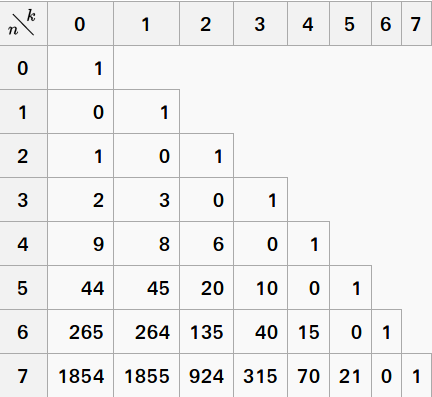
\includegraphics[width=.7\textwidth]{./pictures/3_12.png}
  \caption{Фрагмент таблицы числа встреч}
  \label{fig:312}
\end{figure}

Числа в первом столбце $ \left( k=0 \right) $ показывают число беспорядков (рис. \ref{fig:312}).
Так,
$D_{0, 0} = 1, D_{1, 0} = 0, D_{n+2, 0} = \left( n+1 \right) \left( D_{n+1, 0} + D_{n, 0} \right)$ для неотрицательного $n$.

Выберем $m$ фиксированных элементов из $n$, затем посчитаем число беспорядков оставшихся $n - m$ элементов.
Это будет
$$ \left( n-m \right)! \sum \limits_{k=0}^{n-m} \frac{ \left( -1 \right)^k}{k!}.$$

$$D_{n ,m} =
C_n^m D_{n-m, 0} =
\frac{n!}{m!} \sum \limits_{k=0}^{n-m} \frac{ \left( -1 \right)^k}{k!}.$$
\end{enumerate}

\subsubsection*{3.13}

\textit{Задание.} (Статистика Максвелла-Больцмана). Каждая из $n$ разных частиц наугад попадает в одну из $N$ ячеек.
\begin{enumerate}[label=\alph*)]
\item Найдите вероятность того, что в первой, второй и т.д., N-ой ячейке будет соответственно $n_1, n_2, \dotsc, n_N$ частиц;
\item найдите вероятность $p_k$ того, что данная ячейка содержит $k$ частиц;
\item *докажите, что если $n$ и $N$ стремятся к бесконечности так, что
$$ \frac{n}{N} \rightarrow \lambda,$$
то
$$p_k \rightarrow \frac{ \lambda^k}{k!}e^{- \lambda};$$
\item найдите вероятность того, что в каждой ячейке есть хотя бы одна частица;
\item найдите вероятность того, что занято ровно $r$ ячеек.
\end{enumerate}

\textit{Решение.} В случаях а), б) и д) вероятность желаемого события оценивается по формуле
$$p =
\frac{r}{m}.$$
Для каждой из $n$ разных частиц есть $N$ вариантов попасть в одну из ячеек.
Поэтому по правилу умножения имеем общее количество вариантов $m = N^n$.
Вычислим количество $r$ вариантов, что отвечают каждому из событий, указанных в условии задачи.

\begin{enumerate}[label=\alph*)]
\item Существует $C_n^{n_1}$ способов, которыми можно отобрать $n_1$ частицу в первую ячейку.
Аналогично, количество способов отобрать $n_2$ частицы во вторую ячейку среди $n - n_1$ частицы, которые остались, равно $C_{n-n_1}^{n_2}$.
Подобным же образом отбираются частицы и для других ячеек.
Поэтому событию способствуют
\begin{equation*}
\begin{split}
r =
C_n^{n_1} \cdot C_{n-n_1}^{n_2} \cdot C_{n - n_1 - n_2}^{n_3} \cdot \dotsc = \\
= \frac{n!}{n_1! \left( n-n_1 \right)!}
\cdot \frac{ \left( n-n_1 \right)!}{n_2! \left( n - n_1 - n_2 \right)!}
\cdot \frac{ \left( n - n_1 - n_2 \right)!}{n_3! \left( n - n_1 - n_2 - n_3 \right)!} \cdot \dotsc = \\
= \frac{n!}{n_1! n_2! n_3! \dotsc n_N!}
\end{split}
\end{equation*}
способов.

Тогда вероятность равна
$$p =
\frac{\frac{n!}{n_1! n_2! n_3! \dotsc n_N!}}{N^n} =
\frac{n!}{N^n \cdot n_1! n_2! n_3! \dotsc n_N!};$$

\item сначала нужно отобрать $k$ частиц в фиксированную ячейку
(это можно сделать $C_n^k$ способами),
а потом $n - k$ частиц распределить среди $N - 1$ ячейки
($ \left( N - 1\right)^{n-k}$ способов).
По правилу умножения имеем $r = C_n^k \cdot \left( N-1 \right)^{n-k}$ способов.

Тогда вероятность равна
$$p_k =
\frac{C_n^k \cdot \left( N-1 \right)^{n-k}}{N^n}ж$$

\item *распишем $p_k$:
\begin{equation*}
\begin{split}
p_k =
\frac{C_n^k \left( N-1 \right)^{n-k}}{N^n} =
\frac{n! \left( N-1 \right)^{n-k}}{k! \left( n-k \right)! \cdot N^n} = \\
= \frac{n! \left( N-1 \right)^n}{k! \left( n-k \right)! \cdot N^n \left( N-1 \right)^k} =
\frac{n!}{k! \left( n-k \right)! \left( N-1 \right)^k} \cdot \left( \frac{N-1}{N} \right)^n = \\
= \frac{ \left( n-k \right)! \left( n-k+1 \right) \dotsc n}{k! \left( n-k \right)! \left( N-1 \right)^k} \cdot \left(\frac{N-1}{N} \right)^n =
\frac{ \prod \limits_{i=0}^{k-1} \left( n-i \right) }{k! \left( N-1 \right)^k} \cdot \left( \frac{N-1}{N} \right)^n = \\
= \frac{ \prod \limits_{i=0}^{k-1} \left( \frac{n-i}{N-1} \right)}{k!} \cdot \left( 1 - \frac{1}{N} \right)^n.
\end{split}
\end{equation*}

Умножим и поделим последнюю скобку на $n$.
Получим:
\begin{equation*}
\begin{split}
p_k =
\frac{ \prod \limits_{i=0}^{k-1} \left( \frac{n-i}{N-1} \right)}{k!} \cdot \left( 1 - \frac{ \frac{n}{N} }{n} \right)^n.
\end{split}
\end{equation*}

Возьмём предел полученного выражения при 
$$ \frac{n}{N} \rightarrow \lambda.$$
Получим:
$$ \lim \limits_{ \frac{n}{N} \rightarrow \lambda } p_k =
\lim \limits_{ \frac{n}{N} \rightarrow \lambda }
\left( \frac{ \prod \limits_{i=0}^{k-1} \left( \frac{n-i}{N-1} \right)}{k!} \cdot \left( 1 - \frac{ \frac{n}{N} }{n} \right)^n \right) =
\frac{ \lambda^k}{k!} \exp \left( - \lambda \right);$$

\item вероятность соответственного события вычисляется с помощью формулы включений и исключений:
$P \left\{ \bigcup \limits_{i=1}^m B_i \right\} =
\sum \limits_{i=1}^m P \left\{ B_i \right\} - \\
- \sum \limits_{1 \leq i_1 < i_2 \leq m} P \left\{ B_{i_1} \cap B_{i_2} \right\} + \dotsc + \\
+ \left( -1 \right)^{k-1} \sum \limits_{1 \leq i_1 < i_2 < \dotsc < i_k \leq m} P \left\{ B_{i_1} \cap B_{i_2} \cap \dotsc \cap B_{i_k} \right\} + \dotsc + \\
+ \left( -1 \right)^{m-1} P \left\{ B_1 \cap B_2 \cap \dotsc \cap B_m \right\}$.
Обозначим через $B_i$ событие <<ячейка $i$ не содержит частиц>>.
Тогда $p = 1 - P \left\{ \bigcup \limits_{i=1}^N B_i \right\}$.
Для любых $i = 1, \dotsc, N, \, 1 \leq \\
\leq i_1 < i_2 < \dotsc i_j \leq N$
$$P \left\{ B_i \right\} =
\frac{ \left( N-1 \right)^m}{N^m}, \,
P \left\{ B_{i_1} \cap B_{i_2} \cap \dotsc \cap B_{i_j} \right\} =
\frac{ \left( N-j \right)^m}{N^m}, \,
j = 2, 3, \dotsc, N-1$$
($j$ ячеек являются пустыми; $m$ разных частиц можно разместить в $N - j$ ячейках $ \left( N-j \right)^m$ способами).
Количество слагаемых в соответствующей сумме равно $C_n^j$.
Согласно с формулой включений и исключений имеем окончательный ответ
$$p =
1 - \frac{1}{N^m} \cdot \left[ C_N^1 \cdot \left( N-1 \right)^m - C_N^2 \cdot \left( N-2 \right)^m + \dotsc + \left( -1 \right)^N \cdot C_N^{N-1} \cdot 1^m \right];$$

\item решение задачи разбиваем на два шага: сначала выбираем $r$ ячеек из $N$, которые будут занятыми (это можно сделать $C_N^r$ способами),
а потом размещаем $n$ разных частиц в $r$ ячеек таким образом, чтобы ни одна из них не была пустой ( подобная задача решена в пункте г) по формуле включений и исключений).
Поэтому окончательно имеем
$r =
C_N^r \times \\
\times \left[ r^n - C_r^1 \cdot \left( r-1 \right)^n + C_r^2 \cdot \left( r-2 \right)^n - \dotsc + \left( -1 \right)^{r-1} \cdot C_r^{r-1} \cdot 1^n \right]$.
\end{enumerate}

\addcontentsline{toc}{section}{Дополнительные задачи}
\section*{Дополнительные задачи}

\subsubsection*{3.14}

\textit{Задание.} Каждое из двух чисел $a, b$ наугад выбирают из множества $ \left\{ 1, 2, \dotsc, n \right\}$.
Вычислите вероятность того, что одно из них делится на другое.
Найдите предел этой вероятности при $n \rightarrow \infty$.

\textit{Решение.} Вероятность будет равна
$$P =
\frac{k}{m},$$
где $k$ --- сумма количества делителей каждого числа из множества  $ \left\{ 1, 2, \dotsc, n \right\}$, $m$ --- количество разных пар чисел.

Найдём $m$.
Это будет число комбинаций из $n$ по $2$: $C_n^2$.

Найдём количество множителей натурального числа.
Пусть
$n =
p_1^{ \alpha_1} \cdot p_2^{ \alpha_2} \cdot \\
\cdot \dotsc \cdot p_s^{ \alpha_s}$
--- каноническое разложение на простые множители натурального числа $n$.
Тогда число $ \tau \left( n \right) $ натуральных делителей числа $n$ выражается формулой
$ \tau \left( n \right) =
\left( \alpha_1 + 1 \right) \dotsc \left( \alpha_s + 1 \right)$.

Каждый натуральный делитель $d$ числа $n$
может быть записан в виде
$d = p_1^{ \delta_1} p_2^{ \delta_2} \dotsc p_s^{ \delta_s}$, где $ \delta_i$ ---
целые числа, удовлетворяющие условиям
$ \delta_i \in  \\
\in \left\{ 0, 1, \dotsc, \alpha_i \right\}$
для $i = 1, 2, \dotsc, s$.

Докажем это утверждение.
Пусть $d$ есть какой-либо натуральный делитель $n$.
Так как каждый простой делитель числа $d$
является делителем числа $n$, то ввиду
$n =
p_1^{ \alpha_1} \cdot p_2^{ \alpha_2} \cdot \dotsc \cdot p_s^{ \alpha_s}$
в разложении $d$ на простые множители могут встречаться только числа множества $ \left\{ p_1, \dotsc, p_s \right\}$.
Поэтому число $d$ представимо в виде $d = p_1^{ \delta_1} p_2^{ \delta_2} \dotsc p_s^{ \delta_s}$, где $ \delta_i$,
причём показатели $ \delta_i$ должны удовлетворять условиям
$ \delta_i \in \left\{ 0, 1, \dotsc, \alpha_i \right\}$ для $i = 1, 2, \dotsc, s$.

С другой стороны, если $d$ представимо в виде
$d =
p_1^{ \delta_1} p_2^{ \delta_2} \dotsc p_s^{ \delta_s}$
и показатели удовлетворяют условиям
$ \delta_i \in \left\{ 0, 1, \dotsc, \alpha_i \right\}$
для $i = 1, 2, \dotsc, s$, то
$n =
d \left( p_1^{ \alpha_1 - \delta_1} \dotsc p_s^{ \alpha_s - \delta_s} \right) \left( \alpha_i - \delta_i \geq 0 \right)$,
т.е. $d$ является натуральным делителем числа $n$.

Чтобы найти число всех натуральных делителей числа $n$,
достаточно посчитать число всевозможных упорядоченных наборов
$ \delta_1, \dotsc, \delta_s$, удовлетворяющих условиям
$ \delta_i \in \left\{ 0, 1, \dotsc, \alpha_i \right\}$ для $i = 1, 2, \dotsc, s$.
Ввиду условий $ \delta_i$ может принимать $ \alpha_i + 1$ значение,
выборы различных значений $ \delta_1, \dotsc, \delta_s$
не зависят один от другого
и в силу единственности разложения на простые множители разным наборам соответствуют различные делители $n$.
Следовательно, число всех натуральных делителей числа $n$ равно
$ \left( \alpha_1 + 1 \right) \dotsc \left( \alpha_s + 1 \right)$.

Можно оценить количество делителей числа.
В терминах о-малое,
функция делителей удовлетворяет неравенству для всех $ \epsilon > 0, \, d \left( n \right) = o \left( n^{\epsilon} \right)$.

Тогда имеем вероятность
$$P =
\frac{ \sum \limits_{i=1}^n i^{\epsilon}}{C_n^2} \, \forall \epsilon > 0.$$

\addcontentsline{toc}{section}{Домашнее задание}
\section*{Домашнее задание}

\subsubsection*{3.15}

\textit{Задание.} Докажите, что для произвольных событий A и B
$ P( AB ) = \\
= 1 - P\left( \overline{ A } \right) - P \left( \overline{ B } \right) + P \left( \overline{ A } \, \overline{ B } \right) $.

\textit{Решение.}
$ P( AB ) =
P(A) + P(B) - P \left( A \cup B \right) = \\
= 1 - P \left( \overline{ A }\right) + 1 - P \left( \overline{ B } \right) - \left( 1 - P \left( \overline{ A \cup B } \right) \right) =
1 - P \left( \overline{ A } \right) + 1 - P \left( \overline{ B } \right) - 1 + P \left( \overline{ A } \, \overline{ B } \right) = \\
= 1 - P \left( \overline{ A } \right) - P \left( \overline{ B } \right) + P \left( \overline{ A } \, \overline{ B } \right) $.

\subsubsection*{3.16}

\textit{Задание.} Подбрасывают 4 игральных кубика.
Найдите вероятность того, что на них выпадет одинаковое количество очков.

\textit{Решение.} На выпавшей грани <<первого>> игрального кубика может появиться одно очко, два очка,  $ \dotsc $ , шесть очков.
Аналогичные шесть элементарных исходов возможны при бросании остальных кубиков.
Таким образом, общее число возможных элементарных исходов испытания равно $ 6 \cdot 6 \cdot 6 \cdot 6 = 1296 $.
Эти исходы в силу симметрии кубиков равновероятны.

Благоприятствующие интересующему нас событию
(на всех гранях появится одинаковое количество очков)
являются следующие шесть исходов
(первым записано число очков,
выпавших на <<первом>> кубике,
вторым --- число очков, выпавших на <<втором>> кубике, и т.д.): 1) 1, 1, 1, 1, 2) 2, 2, 2, 2, 3) 3, 3, 3, 3, 4) 4, 4, 4, 4, 5) 5, 5, 5, 5, 6) 6, 6, 6, 6.

Искомая вероятность равна отношению числа исходов, благоприятствующих событию, к числу всех возможных элементарных исходов:
$$ P =
\frac{6}{6^4} = \frac{1}{6^3}.$$

\subsubsection*{3.17}

\textit{Задание.} Группа состоит из r студентов.
Найдите вероятность того, что по крайней мере 2 студента родились в одном и том же месяце (считайте, что все месяцы года являются равновероятными для рождения).

\textit{Решение.} Год имеет 12 месяцев.
День рождения каждого из студентов может приходиться на любой месяц года (12 вариантов).

Если студентов больше чем месяцев ($ r > 12 $), то не существует исходов, при которых в один месяц попадает один человек.
$ P = 0 $.

Рассмотрим случай, когда студентов в группе не больше чем месяцев в году ($ r \leq 12 $).
По правилу умножения существует всего $ n = 12^r $ вариантов размещения дней рождения студентов.
Найдём количество вариантов, когда никакие два студента не имеют день рождения в тот же месяц.
Для этого нужно вычислить количество способов, которыми из 12 месяцев можно выбрать упорядоченное множество из r месяцев.
Используя формулу для размещения из 12 элементов по r, имеем $ A_{12}^r $.
Поэтому
$$ P =
1 - \frac{ A_{ 12 }^r }{ 12^r }.$$

\subsubsection*{3.18}

\textit{Задание.} Сколько людей должно быть в комнате, чтобы вероятность того, что хотя бы двое из присутствовавших родились в один и тот же день года, была большей чем 1/2?

\textit{Решение.} Пусть r --- число людей, и будем считать, что все дни рождения равновероятны.
Вычислим вероятность противоположного события A = {все люди родились в разные дни}.
Число способов, благоприятствующих этому событию --- это число размещений из 365 по r.
Всего же имеется $ n = 365^r $ возможностей распределения дней рождения.
То есть
$$ P(A) =
\frac{A_{365}^r}{365^r}.$$

Вероятность интересующего нас события $ \overline{A} $ тогда равна
$$ P \left( \overline{A} \right) =
1 - P \left( A \right) =
1 - \frac{A_{365}^r}{365^r}.$$

Вычислим вероятность $ P \left( \overline{A} \right) $ для различных значений r.
\begin{equation*}
\begin{split}
r = 5 : P \left( \overline{A} \right) =
1 - \frac{A_{365}^5}{365^5} =
1 - \frac{5! \cdot C_{365}^5}{365^5} = \\
= 1 - \frac{5! \cdot \frac{365!}{5! \cdot 360!} }{365^5} =
1 - \frac{365!}{360! \cdot 365^5} =
1 - \frac{360! \cdot 361 \cdot 362 \cdot 363 \cdot 364 \cdot 365}{360! \cdot 365^5} = \\
= 1 - \frac{361 \cdot 362 \cdot 363 \cdot 364}{365^4} =
1 - \frac{1.72 \cdot 10^10}{1.77 \cdot 10^10} =
1 - 0.97 =
0.03.
\end{split}
\end{equation*}

\begin{equation*}
\begin{split}
r = 10 :
P \left( \overline{A} \right) =
1 - \frac{A_{365}^{10}}{365^{10}} =
1- \frac{10! \cdot C_{365}^{10}}{365^{10}} = \\
= 1 - \frac{10! \cdot \frac{365!}{10! \cdot 355!}}{365^{10}} =
1 - \frac{365!}{355! \cdot 365^{10}} =
0.12.
\end{split}
\end{equation*}

\begin{equation*}
\begin{split}
r = 20 :
P \left( \overline{A} \right) =
1 - \frac{A_{365}^{20}}{365^{20}} =
1 - \frac{20! \cdot C_{365}^{20}}{365^{20}} =
1 - \frac{365!}{345! \cdot 365^{20}} =
0.41.
\end{split}
\end{equation*}

\begin{equation*}
\begin{split}
r = 22 :
P \left( \overline{A} \right) =
1 - \frac{A_{365}^{22}}{365^{22}} =
1 - \frac{365!}{343! \cdot 365^{22}} =
0.48.
\end{split}
\end{equation*}

\begin{equation*}
\begin{split}
r = 23 :
P \left( \overline{A} \right) =
1 - \frac{A_{365}^{23}}{365^{23}} =
1 - \frac{365!}{342! \cdot 365^{23}} =
0.51.
\end{split}
\end{equation*}

При
$ r = 23 $
вероятность по крайней мере одного совпадения равна
$ 0.51 > \\
> 0.5 $,
то есть
$ r = 23 $ ---
наименьшее число, удовлетворяющее условиям задачи.

\subsubsection*{3.19}

\textit{Задание.} Числа $ 1, 2,  \dotsc , n $ размещены в случайном порядке.
Найдите вероятность того, что числа:
\begin{enumerate}[label=\alph*)]
\item 1 и 2;
\item 1, 2 и 3 размещены рядом в указанном порядке.
\end{enumerate}

\textit{Решение.} Пространство элементарных событий $  \Omega$ является множеством всех перестановок множества из n элементов.
Значит $ |\Omega| = n! $.

\begin{enumerate}[label=\alph*)]
\item Поскольку числа 1 и 2 стоят рядом, то их можно рассматривать как одно число (обозначим его $ n + 1 $).
Количество возможных перестановок чисел $ \{ 3, 4,  \dotsc , n + 1 \} $ равно $ \left( n - 1 \right)! $.
Тогда вероятность данного события равна:
$$ P =
\frac{ \left( n - 1 \right)! }{ n! } =
\frac{1}{n};$$

\item поскольку числа 1, 2 и 3 стоят рядом, то их можно рассматривать как одно число (обозначим его $ n + 1 $).
Количество возможных перестановок чисел $ \{ 4, 5,  \dotsc , n + 1 \} $ равно $ \left( n - 2 \right)! $.
Тогда вероятность данного события равна:
$$ P = \frac{ \left( n - 2 \right)!}{ n! } =
\frac{1}{ n (n - 1 ) }.$$
\end{enumerate}

\subsubsection*{3.20}

\textit{Задание.} Экзамен состоит из 10 вопросов, на каждый из которых нужно дать ответ <<да>> или <<нет>>.
Найдите вероятность того, что студент правильно ответил хотя бы на $ 70 \% $ вопросов, выбирая ответ наугад.
Решите задачу, если тест состоит из 30 и из 50 вопросов.

\textit{Решение.} На каждый вопрос есть возможность ответить двумя способами (<<да>> или <<нет>>).

В случае, когда экзамен состоит из десяти вопросов, пространство элементарных событий содержит $ | \Omega | = 2^{10} $ элементов.
Найдём вероятность события А = {студент правильно ответит хотя бы на 70\% вопросов из десяти}.
Ответить правильно хотя бы на 70\% вопросов означает ответить правильно хотя бы на 7 вопросов из 10, т. е. событие А допускает правильный ответ на 7, 8, 9 или 10 вопросов.
На 7 вопросов правильно можно ответить $ C_{10}^7 $ способами.
На 8 вопросов правильно можно ответить $ C_{10}^8 $ способами.
На 9 --- $ C_{10}^9 $.
Аналогично, на 10 вопросов можно дать правильный ответ $ C_{10}^{10} $ способами.
По правилу суммы имеем $ |A| = C_{10}^7 + C_{10}^8 + C_{10}^9 + C_{10}^{10} = \sum \limits_{i=7}^{10} C_{10}^i $.
Тогда вероятность события A равна
$$ P \left( A \right) =
\frac{|A|}{| \Omega |} =
\frac{ \sum \limits_{i=7}^{10} C_{10}^i}{2^{10}}.$$

Аналогично находим вероятность правильного ответа на хотя бы 70\% вопросов из тридцати и пятидесяти.

Когда всего есть 30 вопросов (событие B), то 70\% от них --- это $ 30 \cdot 0.7 = 21$ вопрос.
Тогда
$$ P \left( B \right) =
\frac{ \sum \limits_{i=21}^{30} C_{30}^i}{2^{30}}.$$

Когда всего есть 50 вопросов (событие C), то 70\% от них --- это $ 50 \cdot 0.7 = 35$ вопрос.
Тогда
$$ P \left( C \right) =
\frac{ \sum \limits_{i=35}^{50} C_{50}^i}{2^{50}}.$$

\subsubsection*{3.21}

\textit{Задание.} Список из 4N участников турнира разбито на четыре равные группы.
Найдите вероятность того, что четыре самых сильных участника турнира окажутся в разных группах. 

\textit{Решение.} Найдём сначала количество вариантов, которыми N участников можно выбрать в первую группу.
Для этого достаточно из 4N участников выбрать N, т.е. $ n = C_{4N}^N $.
Выберем того самого сильного участника, который попадёт в первую группу (это можно сделать четырьмя способами).
В эту же группу нужно дополнительно выбрать $ N - 1 $ участника из $ 4N - 4 $ участников, что остались ($ C_{ 4N - 4 }^{ N - 1 } $ способов).
Отсюда следует, что четыре самых сильных участника попадут в разные группы с вероятностью
\begin{equation*}
\begin{split}
p =
\frac{ 4C_{ 4N - 4 }^{ N - 1 } }{ C_{ 4N }^N } =
\frac{ 4 \cdot \frac{ (4N-4)! }{ ( N - 1 )!( 3 N - 3)! } }{ \frac{ (4N)! }{ N!(3N)! } } =
\frac{ 4(4N-4)!N!(3N)! }{ (N-1)!(3N-3)!(4N)! } = \\
= \frac{ 4(4N-4)!(N-1)!N(3N-3)!(3N-2)(3N-1)3N }{ (N-1)!(3N-3)!(4N-4)!(4N-3)(4N-2)(4N-1)4N } = \\
= \frac{ 3N(3N-2)(3N-1) }{ (4N-3)(4N-2)(4N-1) } =
\frac{ 3N(3N-2)(3N-1) }{ 2(4N-3)(2N-1)(4N-1) }.
\end{split}
\end{equation*}

\subsubsection*{3.22}

\textit{Задание.} При игре в покер игрок имеет на руках пять карт из колоды в 52 карты.
Найдите вероятность следующих комбинаций:
\begin{enumerate}[label=\alph*)]
\item <<royal flush>> (десятка, валет, дама, король и туз одной масти);
\item <<straight flush>> (пять карт подряд одной масти, но не <<royal flush>>);
\item <<four of a kind>> (четыре карты одного порядка);
\item <<full house>> (2 карты одинакового порядка и 3 карты одинакового порядка);
\item <<flush>> (пять карт одой масти, но не <<royal flush>> и не <<straight flush>>);
\item <<straight>> (пять карт подряд не все одной масти).
\end{enumerate}

\textit{Решение.} Выбрать 5 карт из 52 можно $ C_{52}^5 $ способами.

\begin{enumerate}[label=\alph*)]
\item Так как есть 4 масти, то десятку можно выбрать четырьмя способами.
Поэтому вероятность выпадения комбинации <<royal flush>> равна
$$ p =
\frac{ C_4^1 }{ C_{52}^5 };$$

\item есть 9 комбинаций пяти карт подряд одной масти.
Так как мастей 4, то этих комбинаций $ 9 \cdot 4 = 36 $.
Поэтому вероятность комбинации <<straight flush>> равна
$$ p =
\frac{ C_{36}^1 }{ C_{52}^5 }.$$
После исключения комбинации <<royal flush>>, получим
$$ p =
\frac{ C_{36}^1 - C_4^1 }{ C_{52}^5 };$$

\item есть 4 масти, в каждой из которых $ 52 : 4 = 13 $ карт.
Есть 13 способов выбрать 4 карты одного порядка.
Так же нужно дополнительно выбрать одну любую карту из оставшихся $ 52 - 4 = 48 $ карт (это 48 способов).
Отсюда имеем, что вероятность комбинации <<four of a kind>> равна
$$ p =
\frac{ C_{13}^1 \cdot C_{48}^1 }{ C_{52}^5 };$$

\item есть карты тринадцати порядков четырёх мастей.
Две карты одного порядка могут иметь любой из тринадцати порядков и любые две из четырёх мастей (это $ C_{13}^1 \cdot C_4^2 $).
Осталось выбрать 3 карты одного порядка. Имеем теперь 12 порядков карт.
Поэтому есть $ C_{12}^1 \cdot C_4^3 $ способов их выбрать.
Итого имеем, что вероятность комбинации <<full house>> равна
$$ p =
\frac{ C_{13}^1 \cdot C_4^2 \cdot C_{12}^1 \cdot C_4^3 }{ C_{52}^5 };$$

\item пять карт одной масти можно выбрать $ 4 \cdot C_{13}^5 $ способами.
Отнимем из этих комбинаций <<royal flush>> и <<straight flush>>.
Получим $ 4 \cdot C_{13}^5 - С_4^1 - C_{36}^1 $.
Поэтому вероятность комбинации <<flush>> равна
$$ p =
\frac{ 4 \cdot C_{13}^5 - С_4^1 - C_{36}^1 }{ C_{52}^5 };$$

\item имея только одну масть есть 9 комбинаций пяти карт подряд.
Каждая из этих пяти карт может быть любой масти.
Главное, чтобы хотя бы одна карта имела масть, отличающуюся от остальных четырёх карт.
Имеем $ 9 \cdot 4^5 $ комбинаций.
Теперь отнимем от них комбинации, где все карты имеют одну масть (их 9).
Поэтому вероятность <<straight>> равна
$$ p =
\frac{ C_9^1 \cdot 4^5 }{ C_{52}^5 }.$$
\end{enumerate}

\subsubsection*{3.23}

\textit{Задание.} Компьютерный центр имеет три процессора, на которые поступило n заданий.
Каждое задание выполняется на наугад выбранном процессоре.
Найдите вероятность того, что ровно один процессор останется незадействованным.

\textit{Решение.} Используем классическое определение вероятности:
$$ P = \frac{m}{k},$$
где m --- число исходов, благоприятствующих осуществлению события, а n --- число всех равновероятных элементарных исходов.

Посчитаем k.
Представим, что процессор --- это ящик.
Положим ящики рядом.
Две соседние стенки назовём <<перегородкой>>, а две крайние стенки не будем рассматривать.
Тогда у нас будет $ 3 - 1 = 2 $ перегородки.
Ситуация выглядит так: Ящик 1 | Ящик 2 | Ящик 3

В эти ящики кладутся предметы (задания).
Итого у нас $ \left( n + 3 - 1 \right) $ позиция --- для n предметов и двух перегородок.
Задание распределения предметов по ящикам равносильно заданию положения перегородок.
Пусть заданы какие-то две позиции для перегородок,
тогда им соответствует некоторое распределение предметов по ящикам
(при этом некоторые ящики могут оказаться пустыми ---
если какая-то перегородка будет на первом месте,
или на последнем, или какие-то перегородки окажутся на соседних местах).
Если же задано некоторое распределение предметов по ящикам,
то в первом окажется $ n_1 $  предмет
(первая перегородка стоит на
$ \left( n_1 + 1 \right) $-ом месте),
во втором ящике --- $ n_2 $ предмета
(вторая перегородка стоит на
$ \left( n_1 + 1 + n_2 +1 \right) $-ом месте)
и так далее, в итоге получим искомые две позиции для перегородок.

Значит, расположить n предметов по разным ящикам можно
$ k = C_{n+2}^{2} $ способом ---
число различных способов распределить n заданий по 6 процессорам,
причём каждый процессор может получить любое количество заданий.

Теперь посчитаем m.
Заданы 2 разных ящика и n предметов.
Нужно расположить предметы по ящикам так, что ни один ящик не будет пустым.

Используем метод перегородок.
Выложим предметы в ряд.
Нужно расставить перегородки так,
чтобы этот ряд распался на две группы (<<группа>> --- это хотя бы один предмет), соответствующих нашим ящикам.

Между n предметами есть $n-1$ место, на которые можно поставить перегородки.
При каждом расположении этих перегородок, получим искомое разбиение на группы --- и в каждой будет хотя бы одни предмет.
Пусть каким-то образом распределены предметы по ящикам, тогда можем определить положения перегородок между объектами,
учитывая количество объектов в каждом ящике.
Значит,
расположить n предметов по двум различным ящикам так,
что ни один ящик не будет пустым,
можно $ C_{n-1}^1 $ способом ---
число способов распределить n задач на два процессора,
причём каждый процессора должен получить не менее одной задачи.
При этом нужно полученное число сочетаний умножить на 3,
так как процессор, который останется без заданий, можно выбрать 3 способами: $ m = 3 \cdot C_{n-1}^1 $.

Искомая вероятность
$$ P =
\frac{ 3 \cdot C_{n-1}^1 }{ C_{n+2}^{2} }.$$

\subsubsection*{3.24}

\textit{Задание.} (Статистика Бозе-Эйнштейна).
Каждая из n одинаковых частиц наугад попадает в одну из N ячеек.
\begin{enumerate}[label=\alph*)]
\item Найдите вероятность того, что в первой, второй и т.д., N-ой ячейке будет соответственно $ n_1, n_2, \dotsc , n_N $ частиц;
\item докажите, что вероятность $ q_k $ того, что в данной ячейке будет k частиц, равна
$$ q_k =
\frac{ C_{ N+n-k-2 }^{ n-k } }{ C_{ N+n-1 }^n };$$
\item докажите, что при $ N > 2 : q_0 > q_1 > q_2 > \dotsc $;
\item докажите, что если n и N стремятся к бесконечности так, что
$$ \frac{ n }{ N } \rightarrow \lambda,$$
то
$$ q_k \rightarrow \frac{ \lambda^k }{ \left( 1 + \lambda \right)^{ k+1 } };$$
\item найдите вероятность того, что ровно r ячеек будут пустыми.
\end{enumerate}

\textit{Решение.}
\begin{enumerate}[label=\alph*)]
\item Разместим частицы в ряд.
Поставим между ними $ N - 1 $ перегородку.
Обозначим частицу символом <<0>>, а перегородку символом <<1>>.
Тогда распределение частиц однозначно характеризуется последовательностью из n нулей и $ N - 1 $ единицы.
Например, последовательность
$ 1000101100001 \dotsc $
означает, что в первую ячейку попало 3 частицы, во вторую --- одна, в третью не попало ни одной частицы, в четвёртую попало 4 частицы и т.д.
Количество способов, которыми можно распределить n частиц, совпадает с количеством разных последовательностей указанного вида.
Последовательность определяется однозначно, если выбрать $ N - 1 $ место из $ n + N - 1$, где будут размещены единицы.
Количество таких комбинаций равно $ | \Omega | = C_{n+N-1}^{N-1} $.

Событию A = { в первой, второй и т.д., N-ой ячейке окажется соответственно $ n_1, n_2, \dotsc , n_N $ частиц}
способствует одно элементарное событие, а именно
$ \omega_0 = \left( n_1, n_2, \dotsc , n_N \right) $.

Таким образом
$$ P(A) =
\frac{1}{C_{n+N-1}^{N-1}};$$

\item вероятность желаемого события оценивается по формуле
$$ q_k =
\frac{r}{| \Omega |}.$$

Аналогично предыдущему пункту $  | \Omega | = C_{n+N-1}^{N-1}  $.

Сначала надо отобрать k частиц в фиксированную ячейку (это можно сделать одним способом), а потом
$ n - k $
частиц распределить среди
$ N - 1 $ ячейки.

Используем метод перегородок.
Разместим все $ n - k $ частиц в ряд.
Чтобы отделить частицы, которые попадут в разные ячейки, поставим между ними $ N - 2 $ перегородки.
Обозначим частицу символом <<0>>, а перегородку символом <<1>>.
Тогда распределение частиц по ячейкам однозначно характеризуется последовательностью из $ n - k $ нулей и $ N - 2$ единиц.
Количество способов, которыми можно распределить
$ n - k $
частиц, совпадает с количеством разных последовательностей указанного вида.
Последовательность определяется однозначно, если выбрать $ N - 2 $ места из $ n - k + N - 2 $, где будут размещены единицы.
Количество таких комбинаций равно $ r = C_{n-k+N-2}^{N-2} $.

Тогда
$$ q_k =
\frac{C_{n-k+N-2}^{N-2}}{C_{n+N-1}^{N-1}};$$

\item найдём вероятность $ q_0 $ того, что в данной ячейке будет 0 частиц.
Вероятность желаемого события оценивается по формуле
$$ q_0 =
\frac{r_0}{| \Omega |}.$$

Аналогично пункту а) $  | \Omega | = C_{n+N-1}^{N-1}  $.

Нужно n одинаковых частиц распределить среди $ N - 1 $ ячейки.

Используем метод перегородок.
Разместим все n частиц в ряд.
Чтобы отделить частицы, которые попадут в разные ячейки, поставим между ними $ N - 2 $ перегородки.
Обозначим частицу символом <<0>>, а перегородку символом <<1>>.
Тогда распределение частиц по ячейкам характеризуется последовательностью из n нулей и $ N - 2 $ единиц.
Количество способов, которыми можно распределить n частиц, совпадает с количеством разных последовательностей указанного вида.
Последовательность определяется однозначно, если выбрать $ N - 2 $ места из $ n + N - 2 $, где будут размещены единицы.
Количество таких комбинаций равно $ C_{n+N-2}^{N-2} $.

Тогда
$$ q_0 =
\frac{C_{n+N-2}^{N-2}}{C_{n+N-1}^{N-1}}.$$

Проверим формулу из пункта б).
Подставим $ k = 0 $.
Получим:
$$ q_0 =
\frac{C_{n+N-2}^{N-2}}{C_{n+N-1}^{N-1}}.$$
Видим, что получили такую же формулу, значит для дальнейшего решения можно использовать её, подставляя вместо k нужное значение.

Упростим:
\begin{equation*}
\begin{split}
q_0 =
\frac{ \frac{ \left( n+N-2 \right)! }{ \left( N-2 \right)! \left( n+N-2-N+2 \right)!  } }{ \frac{ \left( n+N-1\right)! }{\left( N-1 \right)! \left( n+N-1-N+1 \right)!  } } =
\frac{ \left( n+N-2\right)! \left( N-1 \right)!n!}{ \left( N-2 \right)!n! \left( n+N-1 \right)! } = \\
= \frac{ \left( n+N-2 \right)! \left( N-2 \right)! \left( N-1 \right) }{ \left( N-2 \right)! \left( n+N-2 \right)! \left( n+N-1 \right) } =
\frac{N-1}{n+N-1}.
\end{split}
\end{equation*}

Упростим общую формулу:
\begin{equation*}
\begin{split}
q_k =
\frac{ \frac{ \left( n-k+N-2 \right)! }{ \left( N-2 \right)! \left( n-k+N-2-N+2 \right)! } }{ \frac{ \left( n+N-1 \right)!}{ \left( N-1 \right)! \left(n+N-1-N+1 \right)!} } =
\frac{ \left( n-k+N-2 \right)! \left( N-1 \right)!n!}{ \left( N-2 \right)! \left( n-k \right)! \left( n+N-1 \right)!} = \\
= \frac{ \left( n-k+N-2 \right)! \left( N-1 \right) n!}{ \left( n-k \right)! \left( n+N-1 \right)!}.
\end{split}
\end{equation*}

Найдём вероятность $ q_1 $ того, что в данной ячейке будет одна частица:
\begin{equation*}
\begin{split}
q_1 =
\frac{ \left( n-1+N-2 \right)! \left( N-1 \right) n!}{ \left( n-1 \right)! \left( n+N-1 \right)!} = \\
= \frac{ \left( n+N-3 \right)! \left( N-1 \right)! \left( n-1 \right)!n }{ \left( n-1 \right)! \left( n+N-3 \right)! \left( n+N-2 \right) \left( n+N-1 \right) } =
\frac{ \left( N-1 \right) n}{ \left( n+N-2 \right) \left( n+N-1 \right).}
\end{split}
\end{equation*}

Сравним $ q_0 $ и $ q_1 $.
Приведём к общему знаменателю.
Для этого $ q_0 $ умножим на $ \left( n+N-2 \right) $.
Получим:
$$ q_0 =
\frac{ \left( N-1 \right) \left( n+N-2 \right) }{ \left( n+N-1 \right) \left( n+N-2 \right) }.$$

Видим, что $ q_0 $ и $ q_1 $ отличаются только выражением в числителе.
Теперь сравним n и $ \left( n+N-2 \right)$.
По условию задачи $ N > 2 $, поэтому $ N - 2 > 0 $.
Это значит, что $ n + N - 2  > n $, т.е. $ q_0 > q_1 $.

Докажем, что условие выполняется для k-го члена.
Найдём вероятность $ q_{k+1} $ того, что в данной ячейке будет $ k + 1 $ частица:
$$ q_{k+1} =
\frac{ \left( n-k-1+N-2 \right)! \left( N-1 \right) n!}{ \left( n-k-1 \right)! \left( n+N-1 \right)!} =
\frac{ \left( n-k+N-3 \right)! \left( N-1 \right) n!}{ \left( n-k-1 \right)! \left( n+N-1 \right)!}.$$

Сравним полученное выражение с $ q_k $.
В выражении для $ q_{k+1} $ и числитель, и знаменатель меньше: $ n - k + N -3 < n - k + N - 2 $, а также $ n - k - 1 < n - k $.
Отсюда следует, что $ q_k > q_{k+1}$.

Итого, доказали, что условие верно для первого члена $ \left( q_0 > q_1 \right) $.
Также из верности условия для k-го члена вытекает его верность для $ k + 1 $-го.
Отсюда по индукции Пеано следует, что условие верно для любого натурального числа;

\item распишем $ p_k $ (вероятность того, что в данную ячейку попадут k частиц):

\begin{equation*}
\begin{split}
p_k =
\frac{C_{N+n-k-2}^{n-k}}{C_{N+n-1}^n} =
\frac{ \left( N+n-k-2 \right)!n! \left( N-1 \right)!}{ \left( n-k \right)! \left( N-2 \right)! \left( N+n-1 \right)!} = \\
= \frac{ \left( N+n-k-2 \right)! \left( n-k \right)! \left( N-2 \right)! \left( N-1 \right) \prod \limits_{i=0}^{k-1} \left( n-i \right) }{ \left( n-k \right)! \left( N-2 \right)! \left( N+n-k-2 \right)! \prod \limits_{j=1}^{k+1} \left( N+n-j \right) } =
\frac{ \left( N-1 \right) \prod \limits_{i=0}^{k-1} \left( n-i \right) }{ \prod \limits_{j=1}^{k+1} \left( N+n-j \right) }.
\end{split}
\end{equation*}

Поделим числитель и знаменатель на N:
\begin{equation*}
\begin{split}
p_k =
\frac{ \left( 1- \frac{1}{N} \right) \prod \limits_{i=0}^{k-1} \left( \frac{n}{N} - \frac{i}{N} \right) }{ \prod \limits_{j=1}^{k+1} \left( 1+ \frac{n}{N} - \frac{j}{N} \right) } = \\
= \frac{ \frac{n}{N} \left( \frac{n}{N} - \frac{1}{N} \right) \dotsc \left( \frac{n}{N} - \frac{k-1}{N} \right) }{ \left( 1+ \frac{n}{N} - \frac{1}{N} \right) \left( 1+ \frac{n}{N} - \frac{2}{N} \right) \dotsc \left( 1+ \frac{n}{N} - \frac{k+1}{N} \right) } =
\frac{ \lambda^k}{ \left( 1+ \lambda \right)^{k+1}};
\end{split}
\end{equation*}

\item вероятность желаемого события оценивается по формуле
$$ p =
\frac{r}{| \Omega |}.$$

Как и в пункте а) имеем общее количество вариантов $ | \Omega | = C_{n+N-1}^{N-1} $.
Вычислим количество вариантов r, которые отвечают событию, указанному в условии задачи.

Решение задачи разбиваем на два шага:
сначала выбираем $ N - r $ ячеек из N, которые будут занятыми (это можно сделать $ C_{N}^{N-r} $ способами),
а затем размещаем n одинаковых частиц в $ N - r $ ячеек таким образом, чтобы ни одна их них не была пустой.
Поскольку все частицы одинаковы, то в каждую ячейку можно заранее поместить по одной частице.
В этом случае задача сводится к распределению $ m - \left( N - r \right) = m - N + r $ частиц на $ N - r $ ячеек.

Используем метод перегородок.
Разместим все частицы в ряд.
Чтобы отделить частицы, которые будут находиться в разных ячейках, поставим между ними $ N - r - 1 $ перегородку.
Обозначим частицу символом <<1>>, а перегородку символом <<0>>.

Тогда распределение частиц по ячейкам характеризуется последовательностью из $ m - N + r $ нулей и $ N - r - 1 $ единицы.
Количество способов, которыми можно распределить $ m - N + r $ частиц, совпадает с количеством разных комбинаций указанного вида.
Последовательность определяется однозначно, если выбрать $ N - r - 1 $ мест из
$ \left( m - N + r \right) + \left( N - r - 1 \right) = \\
= m - N + r + N - r - 1 = m - 1 $,
где будут стоять единицы.
Количество таких комбинаций равно $ C_{m-1}^{N - r - 1} $.

Поэтому окончательно имеем $ r = C_{N}^{N-r} \cdot C_{m-1}^{N - r - 1} $.

Тогда вероятность указанного события равна
$$ p =
\frac{C_{N}^{N-r} \cdot C_{m-1}^{N - r - 1}}{C_{n+N-1}^{N-1}}.$$
\end{enumerate}
